%% LyX 2.3.0 created this file.  For more info, see http://www.lyx.org/.
%% Do not edit unless you really know what you are doing.
\documentclass[english]{article}
\usepackage[T1]{fontenc}
\usepackage[latin9]{inputenc}
\setlength{\parskip}{\smallskipamount}
\setlength{\parindent}{0pt}
\usepackage{amsmath}
\usepackage{graphicx}
\usepackage{setspace}
\onehalfspacing

\makeatletter
%%%%%%%%%%%%%%%%%%%%%%%%%%%%%% Textclass specific LaTeX commands.
\newcommand{\lyxaddress}[1]{
	\par {\raggedright #1
	\vspace{1.4em}
	\noindent\par}
}

\makeatother

\usepackage{babel}
\begin{document}

\title{The Langmuir Model}

\author{Wei Tian}
\maketitle

\lyxaddress{TSMC}
\begin{abstract}
\noindent In this document, a feature scale model is developed and
used for recipe tuning. The detailed physical mechanisms and numerical
algorithms are introduced and discussed.
\end{abstract}

\section{Introduction - Langmuir Model}

Langmuir model is a comprehensive model simulating the plasma etching
processes. It consists of three sub-models, reactor model, sheath
model and feature model. Reactor model simulates the plasma in the
reactor scale, which is typically 30 to 50 cm.

\section{File Structure}

Langmuir model is organized as a collection of three sub-models and
designed to use solvers as shared as possible. The file structure
is shown in the figure below, 

\begin{figure}
\begin{centering}
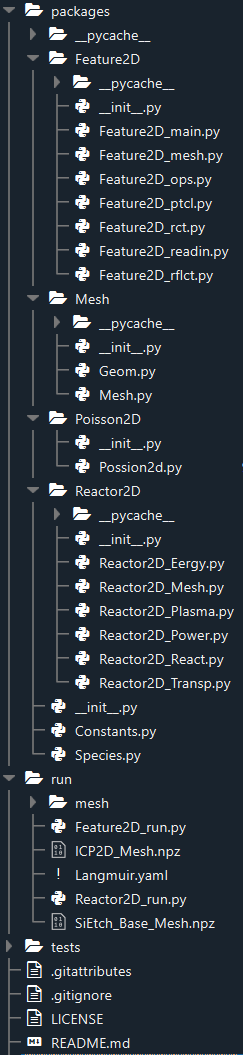
\includegraphics[scale=0.8]{Figures/Dir_Tree}
\par\end{centering}
\caption{The directory/file tree structure for Langmuir model. }
\end{figure}

Within the root directory, there are $packages$, where all the model
are placed, $run$, where applications/cases are run, and $tests$,
where model tests are tested and stored. License and Readme files
are placed in the root directory. Within the $packages$, $Reactor2D$,
$Sheath2D$ and $Feature2D$ directories contains model files for
each model, respectively. File naming follows the convention, $model\:name+2D+module\:name$.
$Constants.py$ and $Species.py$ are shared with all the three models,
so they are placed in the $packages$ level. As for its name, $Constants.py$
defines all constats, while $Species.py$ defines all species and
their properties. These are predefined varables, which are not supposed
to be changed or edited by users. $Mesh$ directory contains $Geom.py$
and $Mesh.py$ to create structured mesh, which in principle can be
used for any model requiring structured mesh, not limited to Langmuir
model. The $Mesh$ module can be either imported to each model or
used as a standalone one. When using as a standalone module, $Mesh$
saves all the information as $mesh.npz$ file. In reactor model, both
field module and transport module require a solver of Poisson-like
equation, therefore $Poisson2D$ is created at this level and works
as a general equation solver. The Poisson solver is also not limited
to Langmuir model. Within the $run$ directory, model run files are
placed. $Langmuir.yaml$ file serves as input file as all-in-one for
all three models. Within $tests$ directory, test are used by developers
and stored as benchmarks for the Langmuir model.

\section{Geometry and Mesh}

\subsection{Geometry}

\subsection{Mesh}

\section{Poisson Equation}

\subsection{Explicit Poisson's equation}

With explict method, the potenital in the Poisson's equation is determined
by the current charge density, which is impacted by the prevous potential.
\[
-\nabla\cdot\varepsilon\nabla\phi(t)=e(\sum_{ion}n_{i}(t)-n_{e}(t))
\]
\[
-\nabla\cdot\varepsilon\nabla\phi(t+\Delta t)=e(\sum_{ion}n_{i}(t+\Delta t)-n_{e}(t+\Delta t))
\]
\[
\dfrac{\partial n_{e,i}}{\partial t}=D_{e,i}\nabla^{2}n_{e,i}(t)\pm\nabla\cdot(\mu_{e,i}n_{e,i}(t)\nabla\phi(t))+S_{e}(t)
\]

\[
n_{e,i}(t+\Delta t)=n_{e,i}(t)+\Delta t\times f_{e,i}(\phi(t))
\]
\[
-\nabla\cdot\varepsilon\nabla\phi(t+\Delta t)=F(\phi(t))
\]

where
\[
\phi=potenital
\]
\[
\varepsilon=permittivity
\]
\[
e=elementary\:charge
\]

\[
n_{e,i}=electron,ion\:density
\]
\[
\mu_{e,i}=electron,ion\:mobility
\]

with the derivation above, the future potential is determined by the
current potenital.

\subsection{Semi-implicit electron with predictor-corrector ions}

The timestep is limited to as small as a few picoseconds, which is
not practical for any useful simulations. Implicit method can theoretically
remove the limit of the timestep, with the cost of solving for the
reversed matrix. The matrix solver could be much expensive as well.
A semi-implict method is, therefore, proposed to increase the timestep
and meanwhile reduce the cost of matrix solver. The principal is shown
as below, 
\[
-\nabla\cdot\varepsilon\nabla\phi(t+\Delta t)=e(\sum_{ion}n_{i}(t+\Delta t)-n_{e}(t+\Delta t))
\]
\[
\dfrac{\partial n_{e}}{\partial t}=D_{e}\nabla^{2}n_{e}(t)-\nabla\cdot(\mu_{e}n_{e}(t)\nabla\phi(t+\Delta t))+S_{e}(t)
\]
\[
n_{e}(t+\Delta t)=n_{e}(t)+\Delta t\times f_{e}(\phi(t+\Delta t))
\]
\[
\dfrac{\partial n_{i}}{\partial t}=D_{i}\nabla^{2}n_{i}(t)+\nabla\cdot(\mu_{i}n_{i}(t)\nabla\phi(t))
\]
\[
n_{i}(t+\Delta t)=n_{i}(t)+\Delta t\times f_{i}(\phi(t))
\]
\[
-\nabla\cdot\varepsilon\nabla\phi(t+\Delta t)=e(\sum_{ion}[n_{i}(t)+f_{i}(\phi(t))]-[n_{e}(t)+f_{e}(\phi(t+\Delta t))])
\]
\[
-\nabla\cdot\varepsilon\nabla\phi(t+\Delta t)=
\]
\[
e(\sum_{ion}[\underline{n_{i}(t)+\Delta t\times f_{i}(\phi(t))}]-\Big[\underline{n_{e}(t)+\Delta t\times S_{e}(t)+\Delta t\times D_{e}\nabla^{2}n_{e}(t)-\Delta t\times\nabla\cdot(\mu_{e}n_{e}(t)\nabla\phi(t+\Delta t))}\Big])
\]
\[
-\nabla\cdot\varepsilon\nabla\phi(t+\Delta t)+e\times\Delta t\times\nabla\cdot(\mu_{e}n_{e}(t)\nabla\phi(t+\Delta t))=F(n_{e,i}(t),\phi(t))
\]
\[
\Big[\underline{-\nabla\varepsilon\cdot\nabla\phi(t+\Delta t)-\varepsilon\nabla^{2}\phi(t+\Delta t)}\Big]+\Big[\underline{(e\mu_{e}\Delta t)\nabla n_{e}(t)\cdot\nabla\phi(t+\Delta t)+(e\mu_{e}\Delta t)n_{e}(t)\nabla^{2}\phi(t+\Delta t)}\Big]
\]
\[
=F(n_{e,i}(t),\phi(t))
\]
\[
[\underline{(e\mu_{e}\Delta t)n_{e}(t)-\varepsilon}]\nabla^{2}\phi(t+\Delta t)+[\underline{(e\mu_{e}\Delta t)\nabla n_{e}(t)-\nabla\varepsilon}]\cdot\nabla\phi(t+\Delta t)=F(n_{e,i}(t),\phi(t))
\]
\[
\underline{A(n_{e}(t))}\nabla^{2}\phi(t+\Delta t)+\underline{\nabla B(n_{e}(t))}\cdot\nabla\phi(t+\Delta t)=F(n_{e,i}(t),\phi(t))
\]
\[
underline-emphasis
\]

The electron density is solved using implicit method, where the future
electron density is determined by the future potential, while the
ion density is still solved using explicit method, where the future
ion density is determined by the current potential. In this scenario,
electron denisty and potential get quickly convergent with large timestep.
A further attension needs to be payed to the ion density, which could
oscillate. The predictor-corrector method is used for ion density.
\[
\tilde{n}_{i}(t+\Delta t)=n_{i}(t)+\Delta t\times f_{i}(n_{i}(t),\phi(t))
\]
\[
n_{i}(t+\Delta t)=n_{i}(t)+\Delta t\times\dfrac{1}{2}(f_{i}(n_{i}(t),\phi(t))+f_{i}(\tilde{n}_{i}(t+\Delta t),\phi(t+\Delta t)))
\]


\subsection{Semi-implicit Poisson's equation}

The ion density can use implicit method as well. In this case, 
\[
-\nabla\cdot\varepsilon\nabla\phi(t+\Delta t)=e(\sum_{ion}[\underline{n_{i}(t)+f_{i}(\phi(t+\Delta t))}]-[\underline{n_{e}(t)+f_{e}(\phi(t+\Delta t))}])
\]
\[
-\nabla\cdot\varepsilon\nabla\phi(t+\Delta t)=e(\sum_{e,i}[\underline{n_{e,i}(t)+f_{e,i}(\phi(t+\Delta t))}]
\]
\[
-\nabla\cdot\varepsilon\nabla\phi(t+\Delta t)=
\]
\[
e(\sum_{e,i}\Big[\underline{n_{e,i}(t)+\Delta t\times S_{e,i}(t)+\Delta t\times D_{e,i}\nabla^{2}n_{e,i}(t)+\Delta t\times\nabla\cdot(q\mu_{e,i}n_{e,i}(t)\nabla\phi(t+\Delta t))}\Big])
\]
\[
-\nabla\cdot\varepsilon\nabla\phi(t+\Delta t)-\sum_{e,i}\Delta t\times\nabla\cdot(eq\mu_{e,i}n_{e,i}(t)\nabla\phi(t+\Delta t))=F(n_{e,i}(t))
\]
\[
[\underline{\sum_{e,i}(eq\mu_{e,i}\Delta t)n_{e,i}(t)-\varepsilon}]\nabla^{2}\phi(t+\Delta t)+[\underline{(e\Delta t)\sum_{e,i}\mu_{e,i}\nabla n_{e,i}(t)-\nabla\varepsilon}]\cdot\nabla\phi(t+\Delta t)=F(n_{e,i}(t))
\]
\[
\underline{A(n_{e,i}(t))}\nabla^{2}\phi(t+\Delta t)+\underline{\nabla B(n_{e,i}(t))}\cdot\nabla\phi(t+\Delta t)=F(n_{e,i}(t))
\]

The future potential is solved directly, which means that the future
potential does not depends on the current potential anymore. All coefficients
in this equation are densities at current time. The second term in
the LHS is probably (not sure, need addtional check) not easy to deal
with. It could be rewritten in explicit form and moved to the RHS.
\[
\underline{A(n_{e,i}(t))}\nabla^{2}\phi(t+\Delta t)+\underline{\nabla B(n_{e,i}(t))}\cdot\nabla\phi(t+\Delta t)=F(n_{e,i}(t))
\]
\[
\underline{A(n_{e,i}(t))}\nabla^{2}\phi(t+\Delta t)=F(n_{e,i}(t))+\underline{\nabla B(n_{e,i}(t))}\cdot\nabla\phi(t)
\]
\[
\underline{A(n_{e,i}(t))}\nabla^{2}\phi(t+\Delta t)=F(n_{e,i}(t),\phi(t))
\]

Now the Poisson's equation retains its Lapalacian form, with the source
term depending on current potential. The same technique can be applied
to Sec. 3.2 as well.

\section{Feature Model}

\subsection{Introduction}

\begin{onehalfspace}
The Langmuir Feature Model uses particle-based Monte Carlo methods
to simulate the evolution of etch features when exposed to plasma
discharges. The model uses pseudo-particles to represent the incoming
species, including electron, ions and neutral particles. All these
pseudo-particles are tracked for their trajectories and interactions
with materials. The materials in the model are represented by a structured
mesh of voxels or cubes. Each voxel or cube represents a macro solid
material, which consists of hundreds of atoms or molecules. The mesh
can be initialized in an arbitrary shape with surface conditions,
which may include multiple materials and features within the each
domain. This allows the simulation of complex structures and steps
in the fabrication process, such as finFET structure. 

A pseudo-particle is also a macro particle, which consists of atoms
or molecules with the same number as in the materials. The pseudo-particles
are launched with specified flux, angle and energy, which are often
derived from a reactor scale model, which is, within the Langmuir
Model, the Langmuir Reactor Model. Without the reactor model, the
Langmuir Feature Model can also self generate generic functions of
flux, angle and energy. The coupling of feature scale model to reactor
scale model allows the Langmuir Model to explore the process recipe
with the etch result, or to be used to study fundamental physics.
This versatility makes the Langmuir Model a strong tool for recipe
tuning and optimization, as well as new physics investigation.
\end{onehalfspace}

\subsection{Mesh - 2D}

\begin{onehalfspace}
The mesh in Langmuir Feature Model is constructed in 2D space, in
which $(x,z)$ are used to represent the 2D coordinates and infinity
is assumed in $y$ direction. The model discretizes the 2D space into
a rectangular computational cells. The cell center is marked as a
node, which determines the location $(x,z)$ of the cell. Each cell
has a volume of $\Delta x\times\Delta z$, where $\Delta x$ and $\Delta z$
are the resolutions in $x$ and $z$ directions, respectively. Usually,
square cells, where $\Delta x=\Delta z$, are used. Non-square cells,
which are used for high aspect ratio domain for memory saving, need
future test and validation. The computational complexity increases
with reducing resolution as approximately $O(n^{3})$, where $n$
is the number of cells per side in the simulation domain. The choice
of resolution also affects the time weighting of each pseudo-particle,
which will be described later.

Each cell, representing a solid material, is assigned a material property.
The most commonly used materials, Such as $Si$ and $SiO_{2}$, in
the Langmuir Feature Model are pre-defined in the database coming
along with the model. If not found in the database, the materials
can be defined by the user. The materials are used for the chemical
reactions. It is important to respect stoichiometry, and most materials
are defined as elements or compounds to facilitate this, but there
is no inherent limitation on the material properties in the model.
It means that arbitrary materials can be built upon simulation request.
In that case, the user is responsible for the validity of the physics
and chemistry represented by the model. An example of an arbitrary
material definition is ``\textit{Photo Resist}'', which is commonly
used as a etching mask. ``\textit{Photo Resist}'' is a polymer with
multiple elements and complicated structures, where a long chain of
molecules could surpass the cell size. It is okay for these resists
to have varying chemistries and properties, and it is not always possible
or necessary to capture their stoichiometry accurately.

The basic element in the mesh is a cell, which is assigned a single
material and not dividable. Each solid cell in the mesh is assumed
to have the same atomic denisty, $\rho\;cm^{-3}$, which is typically
$5.0\times10^{22}\;cm^{-3}$ for $Si$ and $2.3\times10^{22}\;cm^{-3}$
for $SiO_{2}$. This density is a user input and used to calculate
number of atoms per cell, 
\[
N_{cell}=\Delta x\times\Delta z\times\rho
\]
 Because all cells contain a single (usually stoichiometric) material,
but are represented as having the same volume and denisty, it is important
to keep in mind that all materails in the Langmuir Feature Model represent
average behaviors of their respective coupounds. The Langmuir Feature
Model is designed to address the nano-scale feature during the fabrication
process, but not able to resolve the inter-atomic interactions. To
apply the model within the valid window, the user should make sure
that $N_{cell}\gg1$, which will not be automatically checked in the
model. 
\end{onehalfspace}

\subsection{Pseudo-Particle}

\subsubsection{Definition of the pseudo-particle}

Simulating a single ion or radical coming to the feature is not practical
due to the huge computational cost. During a typical etching process,
the ion flux coming to the wafer is of $10^{16}\;cm^{-2}s^{-1}$,
while radical flux of $10^{18}\;cm^{-2}s^{-1}$. In a feature domain
of $100nm\times100nm$ for a process of $10s$, there are$10^{7}$
ions and $10^{9}$ radicas needed to be launched and tracked, which
is clearly beyond the capability of any existing computer or cluster.
Instead of a single particle, a macro-particle called pseudo-particle
and designed like the material cell, is used in the Langmuir Feature
Model. A pseudo-particle consists of $N_{cell}$ identical particles,
which could be electorn, ions, neutals or even photons. Each pseudo-particle
is assigned the properties of a single species and not dividable.
The number density of a pseudo-particle matches the material cell
so that any reactions occur between them are balanced and act as single-particle
reactions.

\subsubsection{Particle Launch}

In a time period $T$, the total launched pseudo-particles, $N_{particle}\times N_{cell}$,
needs to match the total fluence, $Flux\times Aera\times T$, into
the domain. In average, each pseudo-particle occupies a time duration
of 
\[
\Delta t=\dfrac{N_{cell}}{Flux\times Area}
\]
By considering the average velocity of the pseudo-particle and the
domain of the feature, the life time of a pseudo-particle is about
\[
t_{life}=\dfrac{L\times N_{reflect}}{V_{particle}}
\]
where $L$ is the characterstic length of the domain, $L<\sqrt{width^{2}+height^{2}}$,
$N_{reflect}$ is the number of reflections experienced by the pseudo-particle,
$N_{reflect}<10$ for most scenarios, $V_{particle}$ is the average
speed of the pseudo-particle, $t_{life}$ is the lifetime of a pseudo-particle.
Let us put those numbers into an example case. $L=100\:nm$ for a
domain of $100\:nm\times100\:nm$, $N_{reflect}=10$, and $V_{particle}=500\:m/s=500\:nm/ns$
at room temperature. The resulting $t_{life}=2\:ns$ is far smaller
than typical $\Delta t=100\:ns$. It means that a pseudo-particle
is lauched and gets dead before next pseudo-particle is launched,
which indicates that no interaction of pseudo-particles is necessary
to be taken into account. The only interacting object of a pseudo-particle
is the material cell. The summary of the important assumptions can
be seen as below:
\begin{itemize}
\item Pseudo-particles uniformly enter the feature. This indicates that
each pseudo-particle occupies exact $\Delta t$, defined as above.
\item A pseudo-particle entering the feature is a rare event. This implies
that each pseudo-particle event is instantaneous compared to the time
between incoming pseudo-particle. Pseudo-particles do not interact
with each other.
\item The number of total pseudo-particle entering the feature per area
and per time is exactly the same as the flux. This ensures that the
overall effects of total pseudo-particles well align with the physics
requirements.
\end{itemize}
The first assumption can be argued as the real entering events could
follow Poisson's distribution more than uniform distribution. Even
under the assumption of Poisson's distribution, you could find the
event of two pseudo-particles entering the feature with overlap in
time is rare. Compared to millions of pseudo-particles launched in
a simulation, the first two assumptions together still hold. 

\subsubsection{Particle Tracking without E-field}

In the serial version of Langmuir Feature Model, all pseudo-particles
are launched in sequence and particle tracking is only applied to
a single particle each time. In the terms of memory management, a
memory space is created initially for a single pseudo-particle. When
a pseudo-particle dies, a new pseudo-particle can reuse the memory
space by updating the particle properties, such as position and velocity.
The pseudo-particles are by default launched from the top boundary
fo the domain. The initial position of pseudo-particle is randomly
picked. The velocity vector, consisting of speed and angle w.r.t.
$x=0^{+}$, is chosen randomly from the given distribution. The given
distribution could be either generated from the feature model itself,
or from the IAEDF generated from the Langmuir Reactor Model. 

Without E-field, a pseudo-particle is not accelerated during the flight.
It means that the pseudo-particle follows the line--of-sight trajectory.
Although the geometry is meshed to grids, the pseudo-particle advances
in continous space. Newton's equations are solved for the trajectory,
\[
\vec{r}=\vec{r}+\vec{v}\times dt
\]

where $\vec{v}$ and $\vec{r}$ are the velocity and position of the
pseudo-particle, respectively. $dt$ is the flight timestep, which
is far smaller than the simulation timestep. Instead of integrating
over flight timestep $dt$, a advancing step, $\Delta L$ , is used
in Langmuir Feature Model,
\[
\vec{r}=\vec{r}+\vec{v}_{unit}\times\Delta L
\]

where $\vec{v}_{unit}$ is the normalized unit vector of the velocity
and $\Delta L$ is the advance step. Typical $\Delta L$ is constant
and set to be about the resolution of the mesh. Larger $\Delta L$
definitely reduces the computing time. A varying $\Delta L$, which
is determined by the position, can be used and will be discussed separately.
 

\subsubsection{Particle Tracking with E-field}

When E-field is taken into account, velocity for charged particles
is not constant anymore. Full Newton's equations need to be solved,
\[
\vec{v}(t+dt)=\vec{v}(t)+\dfrac{q\vec{E}}{m}dt
\]
\[
\vec{r}=\vec{r}+\vec{v}\times dt
\]

where $\vec{E}$ is the E-field, $q$ is the particle charge, and
$m$ is the particle mass. In the feature model, E-field is a function
of position and changes with deposited surface charges. Within the
tracking of a single particle, E-field does not change with time.
Therefore, Newton's equations can be solved using spacestep instead
of timestep,
\[
\vec{v}(\vec{r}+d\vec{r})=\vec{v}(\vec{r})+\dfrac{q\vec{E}}{m}\times\dfrac{\Delta L}{abs(\vec{v})}
\]
\[
\vec{r}=\vec{r}+d\vec{r}
\]
\[
d\vec{r}=\vec{v}_{unit}\times\Delta L
\]

The chosen of $\Delta L$ depends on the spatial variation of E-field.
In general, if the gradient of E-field is small, $\Delta L$ can be
increased; vice versa. In most cases, $\Delta L$ should not be larger
than the resolution of the mesh.

\subsubsection{Ray Tracing}

To be added.

\subsection{Particle-Materials Interactions}

\subsubsection{Hit Check}

When the particle is tracked by step advance algorithm, particle-materail
collision needs to be checked. In Langmuir Feature Model, there is
no volume assinged to the pseudo-particle, which means that particle
trajectory is an 1D line. At a fixed time, the pseudo-particle is
a point without any dimemsions. When the pseudo-particle gets inside
a material cell, the model flags a ``Hit''. ``Inside a cell''
means that the position $(x,z)$ of the particle lies within the boundary
of the cell,
\[
C_{left}<x<C_{right}
\]
 
\[
C_{bottom}<z<C_{top}
\]
where $C_{left}$, $C_{right}$, $C_{bottom}$ and $C_{top}$ are
the four boundaries for a cell. In the program, in stead of checking
the four boundaries, the particle is mapped onto the computational
mesh of materials using, 
\[
i=int(x-0.5\Delta x)
\]
\[
j=int(z-0.5\Delta z)
\]

It means that the particle is now within the cell $C(i,j)$. If $C(i,j)$
is vacuum, then the particles continues to advance. Otherwise, the
particle is considered to hit the material cell, $C(i,j)$. 
\end{document}
